\documentclass{ctexart}

\usepackage[a4paper,top=2.54cm,bottom=2.54cm,left=3.18cm,right=3.18cm]{geometry}
\usepackage{ctex}
\usepackage{mathtools}
\usepackage{amsmath}
\usepackage{minted}
\usepackage{tikz}
\usepackage{float}
\usepackage{hyperref}

\title{简单流体模拟算法(魔改版)}
\author{TAs}

\begin{document}

\maketitle

\section{问题背景}

\label{sec:bg}

本题目讨论的是\textbf{无外力作用的不可压缩流体}的模拟。在接下来对于二维平面的讨论中,认为纵向方向为 x 方向,横向方向为 y 方向。

\section{\sout{数学} 算法概述}

如果将流体的速度场表示为 $\mathbf{u}$,压强场表示为 $p$,不可压缩流体的 Navier–Stokes 方程可以表示为:

\begin{equation}
\begin{split}
\label{eq:base}
\frac{\partial \mathbf{u}}{\partial t} & = \underbrace{- (\mathbf{u} \cdot \nabla) \mathbf{u}}_1 \underbrace{- \frac{1}{\rho} \nabla p}_2 \underbrace{- \nu \nabla^2 \mathbf{u}}_3 + \mathbf{g} \\
\nabla \cdot \mathbf{u} & = 0
\end{split}
\end{equation}

其中 g 表示外力导致的加速度,由于无外力作用,$\mathbf{g} = \mathbf{0}$。其他部分的含义分别是:

\begin{description}
  \item[1 Advection] 表示随流体本身的流动,把某一处的速度带到相邻位置
  \item[2 Pressure] 表示局部的压强不均导致的速度变化
  \item[3 Diffusion] 表示因为流体粘度带来的局部的速度扩散
\end{description}

为了求以上方程的数值解,在这里需要用到一个数学结论:\textit{Helmholtz-Hodge 分解} 称任意向量场都可以被唯一分解为以下形式:

\begin{equation}
\label{eq:p-operator}
\mathbf{w} = \mathbf{w_n} + \nabla q
\end{equation}

其中 $q$ 是标量场,垂直于边界的变化率为 0 ($\frac{\partial q}{\partial \mathbf{n}} = 0$),$\mathbf{w_n}$ 是一个无散向量场($\nabla \cdot \mathbf{w_n} = 0$)。我们可以定义算子 $\mathsf{P}$,表示将一个向量场映射到它的无散分量上:$\mathsf{P} \mathbf{w} = \mathbf{w_n}$。将 $\mathsf{P}$ 应用在等式 \ref{eq:base} 两侧:

\begin{equation}
\mathsf{P}(\frac{\partial \mathbf{u}}{\partial t})
= \mathsf{P}(- (\mathbf{u} \cdot \nabla) \mathbf{u} - \frac{1}{\rho} \nabla p - \nu \nabla^2 u)
\end{equation}

其中,由于 $\nabla \cdot \mathbf{u} = 0$,而 $\nabla p$ 本身就是一个梯度场,因此 $\mathsf{P}(\frac{\partial \mathbf{u}}{\partial t}) = \frac{\partial \mathbf{u}}{\partial t}$, $\mathsf{P} (\nabla p = 0)$ \footnote{
  可以认为这个投影过程对应的是:方程右侧除了压强项以外的非零散度造成了流体的局部挤压、拉伸,这会造成不均的压强场,它带来的加速度会让方程右侧的散度整体等于零。损失的速度耗散成了热。
}:

\begin{equation}
\label{eq:simple}
\frac{\partial \mathbf{u}}{\partial t}
= \mathsf{P}(- (\mathbf{u} \cdot \nabla) \mathbf{u} - \nu \nabla^2 u)
\end{equation}

根据方程 \ref{eq:simple} 可以构造数值模拟算法,将连续时间切分为时间片,在每个时间片内分为以下几步:

\begin{itemize}
\item 进行流动(Advection)的模拟,更新速度场
\item 进行速度扩散(Diffusion)的模拟,更新速度场
\item 将速度场投影(Projection)到其散度为 0 的分量上
\end{itemize}

\subsection{$\mathsf{P}$ 算子的计算方法}
\label{sec:p-operator}
对方程 \ref{eq:p-operator} 两侧同时计算散度,由于 $\mathbf{w_n}$ 散度为 0:

\begin{equation}
\nabla \cdot \mathbf{w} = \nabla^2 q
\end{equation}

$\mathbf{w}$ 是已知的,可以直接计算它的散度,因此这是一个关于 $q$ 的泊松方程,在流体边界 $\partial D$ 上的边界条件是 $\frac{\partial q}{\partial \mathbf{n}} = 0$

在解得 $q$ 以后,$\mathbf{w_n} = \mathbf{w} - \nabla q$。

\section{实现细节}

\subsection{场的离散表示和算符实现}

模拟的区域为 $x \in (0, h), y \in (0, w)$,计算中储存的所有场都会被离散化为边长为 1 的正方形的格子,存储在 Numpy 数组中。\texttt{f[x, y]} 被定义为场 $f$ 在第 x \textbf{行},第 y \textbf{列} 的格子\textbf{正中央}的值(见图 \ref{fig:grid})。

\begin{figure}[h!]
  \label{fig:grid}
  \centering
  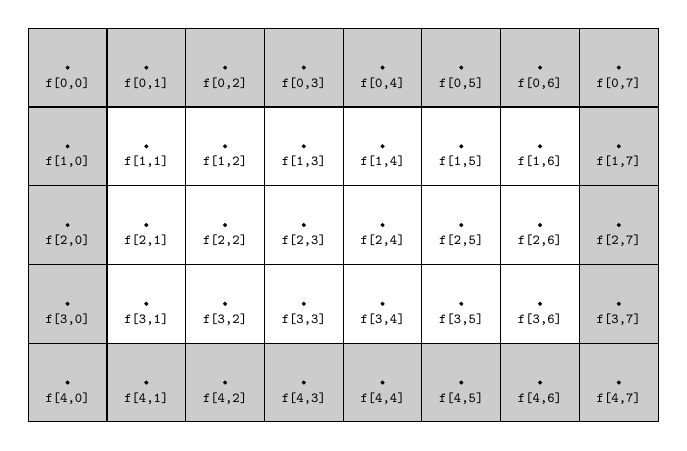
\begin{tikzpicture}
    \foreach \x in {1,...,6}
      \foreach \y in {1,...,3}
        \draw (\x,\y) +(-.5,-.5) rectangle ++(.5,.5);

    \foreach \x in {0,7}
      \foreach \y in {0,...,4}
        \draw [fill=black!20] (\x,\y) +(-.5,-.5) rectangle ++(.5,.5);

    \foreach \x in {1,...,6}
      \foreach \y in {0,4}
        \draw [fill=black!20] (\x,\y) +(-.5,-.5) rectangle ++(.5,.5);

    \foreach \x in {0,...,7}
      \foreach \y in {0,...,4}
      {
        \draw [fill=black] (\x,\y) circle [radius=0.5pt];
        \draw (\x,3.8-\y) node {\tiny \texttt{f[\y,\x]}};
      }
  \end{tikzpicture}

  \caption{场 $f$ 在模拟域上($h = 4, w = 7$)}
\end{figure}

你一共需要存储两个场,在代码模板中已经帮你构造好了:一个速度场 $\mathbf{u}$ (每个格点上是一个二维向量),还有一个表示流体中携带颜料的颜色 $d$ (RBG 三个分量,可以认为是三个分离的标量或者一个三维向量)

为了方便描述边界条件和计算梯度,约定:流体被约束在一个矩形盒子中,在模拟域边上留下长度为 1 的边界(灰色格子)。这些格子的数值都是未定义的,检查时对这些位置的值没有要求,因此可以随意存储任何数值。

据此,我们可以定义梯度和散度算符的离散形式:

\begin{minted}{python}
grad(f, x, y) = [
  (f[x+1, y  ] - f[x-1, y  ]) / 2,
  (f[x  , y+1] - f[x  , y-1]) / 2,
]
div(f_x, f_y, x, y) =
      (f_x[x+1, y  ] - f_x[x-1, y  ]) / 2
    + (f_y[x  , y+1] - f_y[x  , y-1]) / 2
\end{minted}

你可以使用 \texttt{np.roll} 将整个场进行平移,这样可以并行计算整个场的梯度、散度或者拉普拉斯算符应用后的结果。存在的一个问题是:\texttt{np.roll} 对溢出的行为是循环滚动,这样一侧最靠边的值会被移动到另一侧,这是没有实际物理意义的。

根据我们对于模拟域的约定,边界正好分别位于最前两行、最前两列、最后两行、最后两列之间。由于在计算上述算子的时候,最多只需要将场平移一格,因此只需要在每次更新场后将边界外的值覆写,就会解决边界问题。

\subsubsection{边界条件}

选择边界外的值被覆写的内容需要和 Navier-Stokes 方程的边界条件一致。对于速度场,我们选用 No-slip 边界条件:在边界上流体速度为 0。由于我们将格点的值定义为格子正中央的值,因此需要将边界外的格点的值设置成关于边界对称位置的相反的值\footnote{其实四个角落里的值永远不会用到,但是为了实现方便,就不单独处理了}:

\begin{figure}[!h]
  \centering
  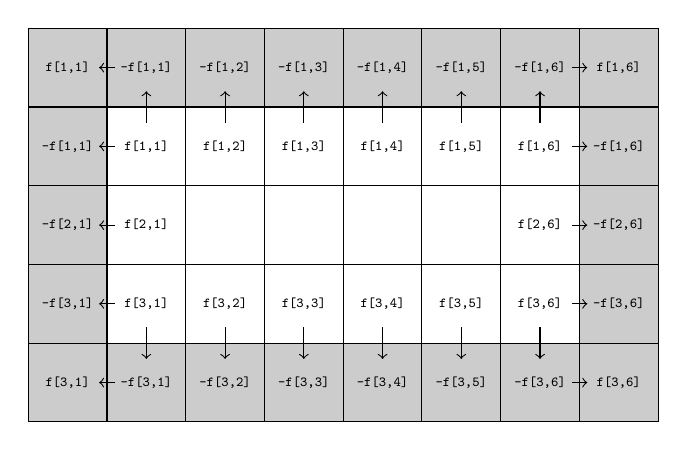
\begin{tikzpicture}
    \foreach \x in {1,...,6}
      \foreach \y in {1,...,3}
        \draw (\x,\y) +(-.5,-.5) rectangle ++(.5,.5);

    \foreach \x in {0,7}
      \foreach \y in {0,...,4}
        \draw [fill=black!20] (\x,\y) +(-.5,-.5) rectangle ++(.5,.5);

    \foreach \x in {1,...,6}
      \foreach \y in {0,4}
        \draw [fill=black!20] (\x,\y) +(-.5,-.5) rectangle ++(.5,.5);

    \foreach \x in {1,...,6}
      \foreach \y in {1,3}
        \draw (\x,4-\y) node {\tiny \texttt{f[\y,\x]}};

    \foreach \x in {1,...,6} {
      \draw (\x,0) node {\tiny \texttt{-f[3,\x]}};
      \draw (\x,4) node {\tiny \texttt{-f[1,\x]}};
    }

    \foreach \x in {1,6}
      \foreach \y in {2}
        \draw (\x,4-\y) node {\tiny \texttt{f[\y,\x]}};

    \foreach \y in {1,...,3} {
      \draw (0,4-\y) node {\tiny \texttt{-f[\y,1]}};
      \draw (7,4-\y) node {\tiny \texttt{-f[\y,6]}};
    }
    
    \draw (0,0) node {\tiny \texttt{f[3,1]}};
    \draw (0,4) node {\tiny \texttt{f[1,1]}};
    \draw (7,0) node {\tiny \texttt{f[3,6]}};
    \draw (7,4) node {\tiny \texttt{f[1,6]}};

    \foreach \x in {1,...,6} {
      \draw [->] (\x,3.3) -- (\x,3.7);
      \draw [->] (\x,0.7) -- (\x,0.3);
    }

    \foreach \y in {0,...,4} {
      \draw [->] (6.4,\y) -- (6.6,\y);
      \draw [->] (0.6,\y) -- (0.4,\y);
    }
  \end{tikzpicture}
  \caption{维护边界条件}
\end{figure}

在 \ref{sec:p-operator} 提及了计算 $\mathsf{P}$ 算子的方法,其中会需要标量场 $q$ 计算梯度。$q$ 的边界条件是垂直于边界方向的变化率为 0,因此需要直接把模拟域内部的值复制到边界外。以上两个过程很类似,可以实现为同一个函数:

\begin{minted}{text}
def set_boundary(field, factor):
  field 的第一行 <- field 的第二行 * factor
  field 的最后一行 <- field 的倒数第二行 * factor
  field 的第一列 <- field 的第二列 * factor
  field 的最后一列 <- field 的倒数第二列 * factor
\end{minted}

在以下过程中中将会多次用到这一函数。

\subsection{Advection}

为了保证算法的稳定性,我们采用隐式方法:根据某一点的速度,找到上一个时间片这一点的流体所处的位置,然后把那里的速度复制过来。同样会随流体流动而移动的东西是流体携带的物质,在这里是颜料:

\begin{equation}
\begin{split}
  \mathbf{u}_{t + \Delta t}(\mathbf{x}) &= \mathbf{u}_t(\mathbf{x} - \mathbf{u}_t(x) \Delta t) \\
  d_{t + \Delta t}(\mathbf{x}) &= d_t(\mathbf{x} - \mathbf{u}_t(x) \Delta t)
\end{split}
\end{equation}

由于 $\mathbf{x} - \mathbf{u}_t(x)$ 不一定正好落在整点上,需要进行插值。我们约定采用 \textbf{双线性插值} (Bilinear Interpolation)

\subsubsection{双线性插值}

简单而言就是对两个方向依次做线性插值:

\begin{figure}[!h]
  \centering

  \begin{tikzpicture}
    \draw (0,0) +(-2,-2) rectangle ++(2,2);
    \node at (0.2,-0.4) [label=above:{$\tilde f(i+\Delta i,j+\Delta j)$},circle,fill,inner sep=1.5pt] {};
    \node at (-2,2.3) {\texttt{f[i,j]}};
    \node at (-2,-2.3) {\texttt{f[i,j+1]}};
    \node at (2,2.3) {\texttt{f[i+1,j]}};
    \node at (2,-2.3) {\texttt{f[i+1,j+1]}};

    \draw [dotted] (-2,-0.4) -- (2,-0.4);
    \node at (-2,-0.4) [label=left:{$\tilde f(i+\Delta i,j)$},circle,draw,inner sep=1.5pt] {};
    \node at (2,-0.4) [label=right:{$\tilde f(i+\Delta i,j+1)$},circle,draw,inner sep=1.5pt] {};
  \end{tikzpicture}
\end{figure}

\begin{equation}
  \begin{split}
    \tilde f(i+\Delta i,j) = & \Delta i \cdot f(i, j) + (1-\Delta i) \cdot f(i + 1, j) \\
    \tilde f(i+\Delta i,j+1) = & \Delta i \cdot f(i, j+1) + (1-\Delta i) \cdot f(i + 1, j+1) \\
    \tilde f(i+\Delta i,j + \Delta j) = & \Delta j \cdot \tilde f(i + \Delta i, j) + (1-\Delta j) \cdot \tilde f(i + \Delta i, j + 1)
  \end{split}
\end{equation}

\subsection{Diffusion}

同样为了保证算法的稳定性,采用隐式方法:

\begin{equation}
(\textbf{I} - \nu \Delta t \nabla^2) \mathbf{u}_{t+\Delta t}(x) = \mathbf{u}_t (x)
\end{equation}

由于我们将 $\nabla ^ 2$ 表示成了矩阵,因此上面这个方程其实是一个线性方程组。

助教在 \texttt{utils.py} 中提供了一个求解以下形式线性方程组的函数:

\begin{equation}
(r \textbf{I} + s \nabla^2) \mathbf{x} = \mathbf{b}
\end{equation}

其中 $\mathbf{x}$ 和 $\mathbf{b}$ 是二维标量场,$r$ 和 $s$ 是参数。

使用方法是调用 \texttt{utils.build\_poisson\_solver(height, width, r, s, factor)}, 其中 \texttt{factor} 的含义和 \texttt{set\_boundary} 中相同。上述调用会返回一个函数 \texttt{f},当你需要求解的时候,你需要将场 $\mathbf{b}$ 形状变为 \textbf{长 \texttt{width * height} 的一维向量},传入 \texttt{f},f 会返回一个 \textbf{长 \texttt{width * height} 的一维向量},代表解得的 $\mathbf{x}$,你需要将其变回原来的形状。

构造函数 \texttt{f} 非常耗时。可以注意到,$\nu$ 是整个模拟中都不会改变的参数,因此上述线性方程组的等式左侧其实永远不变。因此可以在模拟开始前调用一次 \texttt{utils.build\_poisson\_solver},把返回的函数保存起来,之后重复使用即可。

\subsection{Projection}
在 \ref{sec:p-operator} 一节中提到了去除速度场的散度的方法,需要使用你之前实现好的梯度和散度算子。

\textbf{注意!}在使用算子前,请一定要使用 \texttt{set\_boundary} 设置好场的边界值。

此外,\texttt{utils.build\_poisson\_solver} 也可以用来求解 $\mathbf{q}$,返回的函数也同样可以重复使用。

\end{document}
